\problemname{Kängurumamman}

\begin{figure}[!h]
\begin{center}
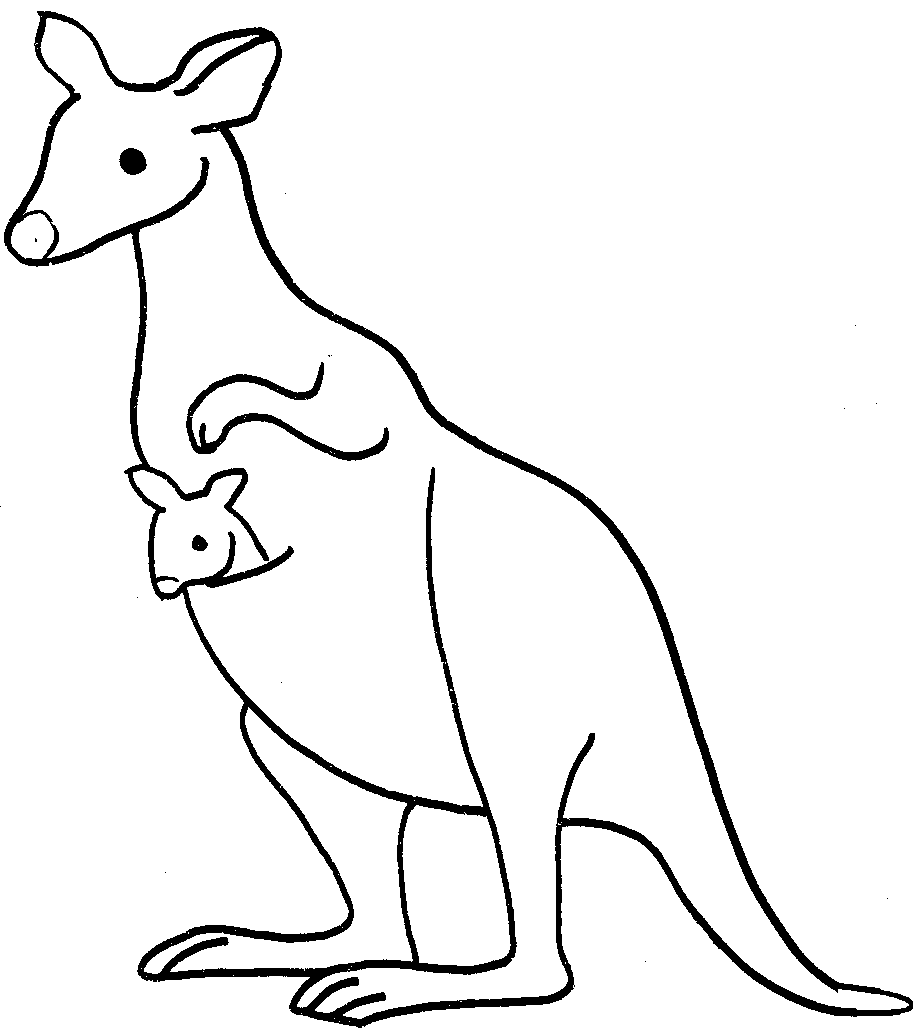
\includegraphics[width=0.3\textwidth]{kangaroo.png} 
\end{center}
\end{figure}

En kängurumamma ska packa ner sina barn i sin pung. Hon har massor med
barn. De två minsta väger bara ett gram var men sen väger varje barn
lika mycket som de två föregående tillsammans. Hennes sex minsta barn
väger alltså 1, 1, 2, 3, 5 och 8 gram.

Mamman orkar bära högst $X$ kilo (och inte ens ett gram mer). Hur många barn kan hon ta med sig?

\section*{Indata}

Indatan består av en rad med ett heltal $X$, där $1\le X \le 1000$, det
maximala antalet kilo mamman orkar bära.

\section*{Utdata}

Programmet ska skriva en rad med ett heltal, det största antalet barn
som tillsammans väger högst $X$ kilo.
